\documentclass[a4paper,USenglish,cleveref,autoref,thm-restate,anonymous]{lipics-v2021}
%This is a template for producing LIPIcs articles. 
%See lipics-manual.pdf for further information.
%for A4 paper format use option "a4paper", for US-letter use option "letterpaper"
%for british hyphenation rules use option "UKenglish", for american hyphenation rules use option "USenglish"
%for section-numbered lemmas etc., use "numberwithinsect"
%for enabling cleveref support, use "cleveref"
%for enabling autoref support, use "autoref"
%for anonymousing the authors (e.g. for double-blind review), add "anonymous"
%for enabling thm-restate support, use "thm-restate"

%\graphicspath{{./graphics/}}%helpful if your graphic files are in another directory

\hideLIPIcs 

\ccsdesc{%
Theory of computation $\rightarrow$ 
Design and analysis of algorithms $\rightarrow$ 
Parameterized complexity and exact algorithms $\rightarrow$ 
Fixed parameter tractability}


% TODO 




\bibliographystyle{plainurl}
\newcommand{\citet}[1]{\cite{#1}}
\usepackage{graphicx}
\urlstyle{rm}
\def\UrlFont{\rm}
\usepackage{graphicx} 
\newif\iflong
\newif\ifshort

% comment the below line out for short version
\longtrue

\keywords{parameterized complexity, NLC-width, rank-width, decision trees, partially defined Boolean formulas}

\usepackage{tikz}
\usepackage{booktabs}
\usepackage[noend]{algpseudocode}
\usepackage{algorithm,algorithmicx}
\newcommand{\NULL}{\textnormal{\texttt{nil}}}
\newcommand{\TRUE}{\texttt{TRUE}}
\newcommand{\FALSE}{\texttt{FALSE}}

\algnewcommand\algorithmicinput{\textbf{Input:}}
\algnewcommand\INPUT{\item[\algorithmicinput]}

\algnewcommand\algorithmicoutput{\textbf{Output:}}
\algnewcommand\OUTPUT{\item[\algorithmicoutput]}

% decision trees and parameters
\newcommand{\DTL}{\probfont{DTS}}
\newcommand{\DTLh}{\probfont{DTD}}
\newcommand{\MSS}{\textup{MSS}}
\newcommand{\MNE}{\min_{\#}}
\newcommand{\GIL}{G^+_I}


\newcommand{\inst}{I}
\newcommand{\MIHS}{\probfont{MIHS}}

% \newcommand{\HD}{\delta}
% \newcommand{\MHD}{\delta_{\max}}
%\newcommand{\DMAX}{D_{\max}}

% \newcommand{\GD}{D}
% \newcommand{\IV}{I}

\usepackage{todonotes}
\presetkeys%
    {todonotes}%
    {inline,backgroundcolor=yellow}{}

%table stuff?
\usepackage{booktabs}
\usepackage{multirow}
%\usepackage{floatrow}

\usepackage{amsthm,amsmath,amssymb}
\usepackage{enumerate,verbatim}
\usepackage{xspace}

\usepackage{tikz,tikz-cd}
\usetikzlibrary{arrows,cd,positioning,shapes,patterns}


\usepackage[draft,author=]{fixme}
\fxsetup{theme=color}
%\newcommand{\todo}[1]{\fxerror{#1}}
\newcommand{\warn}[1]{\fxwarning{#1}}
\renewcommand{\note}[1]{\fxnote{#1}}
\newcommand{\nb}[1]{\todo{\scriptsize #1}}



\newcommand{\SB}{\{\,}
\newcommand{\SM}{\;{|}\;}
\newcommand{\SE}{\,\}}
\newcommand{\PP}{\mathcal{P}}
\newcommand{\QQ}{\mathcal{Q}}
\newcommand{\III}{\mathcal{I}}
\newcommand{\SSS}{\mathcal{S}}
\newcommand{\RRR}{\mathcal{R}}
\newcommand{\DDD}{\mathcal{D}}
\newcommand{\FFF}{\mathcal{F}}
\newcommand{\TTT}{\mathcal{T}}
\newcommand{\VVV}{\mathcal{V}}
\newcommand{\XXX}{\mathcal{X}}

\newcommand{\RR}{\mathcal{R}} 

\newcommand{\Z}{\mathbb{Z}}
\newcommand{\Nat}{\mathbb{N}}
\newcommand{\downcl}[2]{D_{#1}(#2)}
\newcommand{\pref}{P_{\leq^V}}
\newcommand{\suff}{S_{\leq^V}}

\newcommand{\bigoh}{\mathcal{O}}
\newcommand{\littleoh}{o}

 
 


\newcommand{\cc}[1]{{\mbox{\textnormal{\textsf{#1}}}}\xspace}  %% Complexity class
\newcommand{\cocc}[1]{{\mbox{\textrm{co}\textnormal{\textsf{#1}}}}\xspace}  %% Complexity class

\newcommand{\integers}{\mathbb{Z}}
\renewcommand{\P}{\cc{P}}
\newcommand{\NP}{\cc{NP}}
\newcommand{\coNP}{\cc{co-NP}}
\newcommand{\FPT}{\cc{FPT}}
\newcommand{\XP}{\cc{XP}}
\newcommand{\Weft}{{\cc{W}}}
\newcommand{\W}[1]{{\Weft}{{\textnormal[#1\textnormal]}}}
\newcommand{\paraNP}{\cc{paraNP}}
\newcommand{\paraNPs}{\cc{pNP}}


\newcommand{\fpt}{fixed-pa\-ra\-me\-ter trac\-ta\-ble\xspace}

\newcommand{\tuple}[1]{\langle{#1}\rangle}  % Tuple
\newcommand{\pn}[1]{\textsc{#1}}
\newcommand{\hy}{\hbox{-}\nobreak\hskip0pt}

%\newcommand{\citet}[1]{\citeauthor{#1}~\shortcite{#1}\xspace}
\newcommand{\nn}{\mathbb{N}}

\newcommand{\bigO}[1]{\ensuremath{{\mathcal O}(#1)}}
\newcommand{\bigOstar}[1]{\ensuremath{{\mathcal O}^*(#1)}}

\newcommand{\probfont}[1]{\textnormal{\textsc{#1}}}

%\newcommand{\stw}{dependency treewidth}



%\newcommand{\RAPROG}{\probfont{Proportionality Graph Allocation}}
\newcommand{\RAENVG}{\probfont{(Locally) Envy-Free Allocation}}
\newcommand{\RAENVGNL}{\probfont{Envy-Free Allocation}}
\newcommand{\RAENVGL}{\probfont{Locally Envy-Free Allocation}}

\newcommand{\EFA}{\textsc{EFA}}
\newcommand{\LEFA}{\textsc{LEFA}}

\newcommand{\FCGENVPROP}{envy-free}
\newcommand{\FCGENV}{locally envy-free}
\newcommand{\FCGPROP}{proportional}

\newcommand{\AT}{T_A}
\newcommand{\RT}{T_R}
\newcommand{\mundef}{\textup{undef}}
\newcommand{\BS}{\textup{BS}}

\newcommand{\RofRT}{R}
\newcommand{\RTBUN}{\textup{BUN}}
\newcommand{\RTVEC}{\vec{b}}
\newcommand{\RTVECSET}{\mathcal{B}}

\newcommand{\rall}{\alpha}
\newcommand{\itf}{\vec{u}}
\newcommand{\new}[1]{}
\newcommand{\valn}{\beta}
\newcommand{\VR}{\RRR}


\newcommand{\prop}[1]{#1}
\newcommand{\noprop}[1]{}
\newcommand{\bunmin}{\alpha_{\min}}
\newcommand{\bunmax}{\alpha_{\max}}
\newcommand{\propmax}{\beta}
\usepackage{boxedminipage}

\newcommand{\MCC}{\probfont{Multicolored Clique}}

\newcommand{\pbDef}[3]{%
\noindent
\begin{center}
\begin{boxedminipage}{0.98 \columnwidth}
#1\\[5pt]
\begin{tabular}{l p{0.70 \columnwidth}}
Input: & #2\\
Question: & #3
\end{tabular}
\end{boxedminipage}
\end{center}
}

\newcommand{\pbDefP}[4]{%
\noindent
\begin{center}
\begin{boxedminipage}{0.98 \columnwidth}
#1\\[5pt]
\begin{tabular}{l p{0.70 \columnwidth}}
Input: & #2\\
Parameter: & #3\\
Question: & #4
\end{tabular}
\end{boxedminipage}
\end{center}
}


\newcommand{\lc}{l}
\newcommand{\rc}{r}

\newcommand{\reaches}{r}


\newcommand{\CCC}{\mathcal{C}}

\newcommand{\ol}[1]{\overline{#1}}
\newcommand{\Card}[1]{|#1|}
\let\phi=\varphi
\let\epsilon=\varepsilon 
\def\hy{\hbox{-}\nobreak\hskip0pt} 
% Name for our encoding and for the whole approach
\newcommand{\enc}{DT\_pb}
\newcommand{\ench}{DT\_hyb}
\newcommand{\slv}{DT\_rec}
% Subsampling strategies
\newcommand{\stratrand}{RandSelect}
\newcommand{\stratlearn}{TreeSelect}
\newcommand{\stratleaf}{LeafSelect}
\newcommand{\stratinc}{MonotonicSelect}
% Feature reduction
\newcommand{\redcon}{\text{FR}}
\newcommand{\redgreedy}	{$\redcon_{\text{greedy}}$}
\newcommand{\redmaxsat}	{$\redcon_{\text{maxsat}}$}
\newcommand{\redrand}	{$\redcon_{\text{rand}}$}
\newcommand{\reddec}	{$\redcon_{\text{back}}$}

% reduction flags
\newcommand{\redinit}{RI}
\newcommand{\redinc}{RC}

\newcommand{\dif}{\text{\specialfont{diff}}}
\newcommand{\dom}{\text{\specialfont{dom}}}
\newcommand{\siz}{\text{\specialfont{size}}}
\newcommand{\solsize}{\text{\specialfont{sol}}}

\newcommand{\parameter}[1]{\text{\normalfont{\sffamily #1}}}
 

\newcommand{\var}{\text{\specialfont{feat}}}
\newcommand{\feat}{\text{\specialfont{feat}}}
\newcommand{\thres}{\lambda}

\newcommand{\leaf}{\text{\specialfont{leaf}}}



\newcommand{\specialfont}[1]{{\normalfont\slshape #1}}

\newcommand{\nlcw}{\text{\specialfont{nlcw}}}
\newcommand{\rtw}{\text{\specialfont{rtw}}}
\newcommand{\tw}{\text{\specialfont{tw}}}
\newcommand{\cw}{\text{\specialfont{cw}}}
\newcommand{\rw}{\text{\specialfont{rw}}}
\newcommand{\dep}{\text{\specialfont{dep}}}
\newcommand{\ghtw}{\text{\specialfont{ghtw}}}
\newcommand{\htw}{\text{\specialfont{htw}}}




\begin{document}
%\raggedright\pagestyle{empty}\nolinenumbers

\ifshort
\title{Fixed-Parameter Tractability of\\  Learning Small Decision Trees}
\fi
\iflong
\title{Fixed-Parameter Tractability of\\  Learning Small Decision Trees\\(full paper)}
\fi

\author{TODO}{~}{~}{}{}
\authorrunning{~}
\titlerunning{}
\maketitle


%\begin{abstract}
%We consider the NP-hard problem of finding a smallest decision tree which represents a given partially defined Boolean formula. We establish fixed-parameter tractability of the problem with respect to the NLC-width of the instance. We formulate a dynamic programming procedure which utilizes the NLC-decomposition of the instance. For this to work, we establish a succinct representation of partial solutions, so that the space and time requirements of each dynamic programming step remain bounded in terms of the NLC-width.
%\end{abstract}
 
\newpage
\clearpage

\setcounter{page}{1}

\section{Introduction}
Decision trees have proved to be extremely useful tools for the describing, classifying, generalizing data~\cite{Larose05,Murthy98,Quinlan86}. In this paper, we consider decision trees for {\it classification instances (CIs)}, consisting of a finite set $E$ of {\it examples} (also called {\it feature vectors}) over a finite set $F$ of {\it features}. Each example $e\in E$ is a function $e:F\rightarrow \{0,1\}$ which determines whether the feature~$f$ is true or false for $e$.  Moreover, $E$ is given as a partition $E^+ \uplus E^-$ into positive and negative examples. For instance,  examples could represent medical patients and features diagnostic tests; a patient is positive or negative corresponding to whether they have been diagnosed with a certain disease or not. CIs are also called {\it partially} or {\it incompletely defined Boolean functions}, as we can consider the features as Boolean variables, and examples as  truth assignments that evaluate to 0 (for positive examples) or 1 (for negative examples). CIs have been studied as a key concept for the logical analysis of data and in switching theory \cite{BorosCHIKM11,Boros03,BorosGHIK95,BorosIbarakiMakino03,   CramaHammerIbaraki88,IbarakiCramaHammer11,Mccluskey65}.

Because of their simplicity, decision trees are particularly attractive for providing interpretable models of the underlying CI, an aspect whose importance has been strongly emphasized over the recent years~\cite{DarwicheHirth20,DoshivelezKim17,GoodmanFlaxman17,Lipton18,Monroe18}. In this context, one prefers {\it small trees}, as they are easier to interpret and require fewer tests to make a classification. Small trees are also preferred in view of the parsimony principle (Occam’s Razor) since small trees are expected to generalize better to new data~\cite{Bessiere09}. However, finding a small decision tree, as formulated in the following decision problem, is NP-complete~\cite{HyafilRivest76}. 

\begin{quote}
\probfont{Minimum Decision Tree Size (\DTL):} given a CI $E=E^+ \uplus E^-$ and an integer $s$, is there a decision tree with at most $s$ nodes for $E$?
\end{quote}

Given this complexity barrier, we propose a fixed-parameter algorithm for the problem, which exploits the input CI's hidden structure. 

\section{Preliminaries}\label{chap:prelims}

\subsection{Parameterized Complexity}
We give some basic definitions of Parameterized Complexity and refer for a more in-depth treatment to other sources \cite{CyganFKLMPPS15,DowneyFellows13}. Parameterized complexity considers problems in a two-dimensional
setting, where a problem instance is a pair $(I,k)$, where $I$ is the main part and~$k$ is the parameter. A parameterized problem is {\it fixed-parameter tractable} if there exists a computable function $f$ such that instances $(I,k)$ can be solved in time $f(k) \|I\|^{O(1)}$.

\newcommand{\lab}{\lambda}

\subsection{Classification Problems} 
An {\it example} $e$ is a function $e:\feat(e) \rightarrow \{0,1\}$ defined on a finite set $\feat(e)$ of {\it features}. For a set $E$ of examples, we put $\feat(E)=\bigcup_{e\in E} \feat(e)$. We say that two examples $e_1,e_2$ {\it agree} on a feature $f$ if $f \in \feat(e_1)$, $f\in \feat(e_2)$ and $e_1(f)=e_2(f)$. If $f \in \feat(e_1)$, $f \in \feat(e_2)$ but $e_1(f)\neq e_2(f)$, we say that the examples {\it disagree on $f$}.

A {\it classification instance (CI)} (also called a {\it partially defined Boolean function}\ \cite{IbarakiCramaHammer11})
$E=E^+ \uplus E^-$ is the disjoint union of two sets of examples, where for all $e_1,e_2\in E$ we have $\feat(e_1)=\feat(e_2)$. The examples in $E^+$ are said to be {\it positive}; the examples in $E^-$ are said to be {\it negative}.  A set $X$ of examples is {\it uniform} if $X\subseteq E^+$ or $X \subseteq E^-$; otherwise $X$ is {\it non-uniform}.
 
Given a CI $E$, a subset $F\subseteq \feat(E)$ is a {\it support set} of $E$ if any two examples $e_1\in E^+$ and $e_2\in E^-$ disagree in at least one feature of $F$.  Finding a smallest support set, denoted by $\MSS(E)$, for a classification instance $E$ is an NP-hard task~\cite[Theorem 12.2]{IbarakiCramaHammer11}.
 
We define the {\it incidence graph} of $E$, denoted by $G_I(E)$, as the bipartite graph with partition $(E, \feat(E))$ having an edge between an example $e \in E$ and a feature $f\in \feat(e)$ if $f(e)=1$.

\subsection{Decision Trees}
A {\it decision tree} (DT) (or {\it classification tree}) is a rooted tree $T$ with vertex set $V(T)$ and arc set $A(T)$, where each non-leaf node (called a {\it test}) $v\in V(T)$ is labelled with a feature $\feat(v)$, each non-leaf node $v$ has exactly two out-going arcs, a {\it left arc} and a {\it right arc}, and each leaf is either a {\it positive} or a {\it negative} leaf. We write $\feat(T)=\SB v\in V(T) \SM \feat(v) \SE$.

Consider a CI $E$ and a decision tree $T$ with $\feat(T)\subseteq \feat(E)$. For each node $v$ of $T$ we define $E_T(v)$ as the set of all examples $e\in E$ such that for each left (right, respectively) arc $(u,v)$ on the unique path from the root of $T$ to~$v$ we have $e(\feat(v))=0$ ($e(\feat(v))=1$, respectively).  $T$ {\it correctly classifies} an example $e\in E$ if $e$ is a positive (negative) example and $e\in E_T(v)$ for a positive (negative) leaf. We say that $T$
{\it classifies} $E$ (or simply that $T$ is a DT for $E$) if $T$ correctly classifies every example $e \in E$. See Figure~\ref{fig:example} for an illustration of a CI, its incidence graph, and a DT that classifies $E$.

The size of $T$ is its number of nodes, i.e. $|V(T)|$. We consider the following problem.

\pbDef{\probfont{Minimum Decision Tree Size} (\DTL)}{A classification instance $E$ and an integer $s$.}{Is there a decision tree of size at most $s$ for $E$?}

\newcommand{\NO}{\textbf{NO}}
\newcommand{\TsmDT}{(2^{|E|})^{4|E|-1}}
\newcommand{\exam}{\text{\specialfont{exam}}}
\newcommand{\afs}{\textup{TF}}
\newcommand{\afsF}{\textup{TF}_F}
\newcommand{\afsP}{\textup{TF}_P}
\newcommand{\addF}{\oplus}
\newcommand{\SoIF}[1]{I_{#1}}
\newcommand{\SoFF}[1]{F_{#1}}
\newcommand{\anc}{\textit{\textup{anc}}}
\newcommand{\AL}{A}
\newcommand{\red}{r}
\newcommand{\frf}{\alpha}
\newcommand{\rel}{\eta}
\newcommand{\rlstan}[1]{\alpha^s_{#1}}

\section{An FPT-Algorithm for bounded solution size and $\delta_{max}$.}

In the following, let $E$ be a CI and $q\not\in feat(E)$. A {\it decision tree pattern}, or simply a {\it DT pattern}, $T$ is a rooted subcubic tree, where every leaf node is either a {\it positive} or {\it negative} leaf and every non-leaf node is labelled with a feature in $feat(E)\cup \{q\}$. For every node $v$ of a DT pattern $T$, we indicate with $feat_T(v)$ the label associated to that node. Finally we say that an innder node $v\in V(T)$ is a {\it fixed node} if $feat_T(v)\in feat(E)$ and {\it non-fixed} otherwise.

A DT pattern $T'$ is an {\it improvement} for a DT pattern $T$ if $T'=T$ as rooted trees and $feat_{T'}(v)=feat_{T}(v)$ for every fixed node $v$ of $T$. 
A {\it complete improvement} $T'$ of $T$ is an improvement such that $feat(T')\subseteq feat(E)$. 
A {\it threshold assignment} for a DT pattern $T$ is a function $th$ that maps every fixed node $v\in V(T)$ to a natural number $th(v)$. Note that any complete improvement $T'$ of a DT pattern $T$ can be made to a decision tree with a threshold assignment.

Let $T$ be a DT pattern and $th$ be a threshold assignment for $T$, for each node $v$ of $T$ we define the set of examples that arrive at node $v$, $E_T(v)$ as follows: $E_T(v)$ is the set of all examples $e\in E$ such that for each left (right, respectively) arc $(u,w)$ on the unique path from the root of $T$ to~$v$ either $u$ is a fixed node and $(feat(u))(e)\leq th(u)$ ($(feat(u))(e)> th(u)$, respectively) or $u$ is a non-fixed node.
A DT pattern $T$ is {\it valid} for a set of examples $E'\subseteq E$ if there is threshold assignment for the fixed nodes such that for every positive (negative) example $e$, $e\in E_T(v)$ for a positive (negative) leaf $v$.

The definition of $E_T(v)$ is an indication of the behaviour of feature $q$ and of non-fixed nodes. Informally, if any example reaches at a non-fixed node of $T$ then it reach both his children. While no feature in $feat(E)$ can simulate such behaviour for any threshold, $q$ simultaneously cover the two cases a feature with his threshold does not distinguish any two examples. 

\begin{comment}
Given a CI $E$, our aim it to construct a support set $S^*$ for $E$ such that there is a DT $T^*$ for $E$ of size at most $s$ with $feat(T^*)=S^*$.

First of all, we note that we can enumerate all the minimal support sets in fpt-time parametrized by $\delta_{max}$ as follows.

\begin{lemma}[\cite{OrdyniakSzeider21}]
Let $E$ be a CI and let $k$ be an integer. Then there is an algorithm that in time $\mathcal{O}(\delta_{max}(E)^k|E|)$ enumerates all (of the at most $\mathcal{O}(\delta_{max}(E)^k|E|)$) minimal support sets of size at most $k$ for $E$.
\end{lemma}

Let $S$ be a support set for $E$. Consider a DT $T$, we say that a non-leaf node $t$ of $T$ has an {\it unknown feature} for $S$ if $feat(t)\not\in S$; if $feat(t)\in S$ then we say that $t$ has a {\it supported feature}. If a DT $T$ contains an unknown feature for a support set $S$, then it is called a {\it partial DT} for $S$. Otherwise, that is if $T$ does not contain any unknown features for $S$, $T$ is called a {\it supported DT} for $S$. %In a partial DT for $S$, we define $sfeat(T):=feat(T)\cap S$.

The following Lemma express that we can already solve the problem in the case we have a supported DT $T$ for $S$: this is given by the fact a feature assignment $\alpha$ for $T$ is known.

\begin{lemma}[\cite{OrdyniakSzeider21}]\label{lem:dtthres}
Let $E$ be a CI, let $T$ be DT for $S$ of depth $d$ and let $\alpha$ be a feature assignment for $T$. Then, there is an algorithm that runs in time $\bigoh(2^{d^2/2}\|E\|^{1+\littleoh(1)}\log \|E\|)$ and decides whether the pair $(T,\alpha)$ can be extended to a DT for~$E$. 
\end{lemma}
\end{comment}

\subsection{Preprocess}
Let $E$ be a CI and $T$ be a DT pattern. 
For every $v\in V(T)$, we define the set of {\it expected examples} $E_v$ as follows:

\begin{itemize}
\item if $v$ is the root, then $E_v=E$;
\item if $v$ is the left child of a fixed node $v_p$, then $E_v=E_{v_p}[feat(v_p)\leq th_L(v_p)+1]$;
\item if $v$ is the right child of a fixed node $v_p$, then $E_v=E_{v_p}[feat(v_p)> th_R(v_p)-1]$;
\item if $v$ is a child of a non-fixed node $v_p$, then $E_v=E_{v_p}$.
\end{itemize}

Node that the definition of $E_v$ is strictly related with the following: if $v$ is a fixed node, let $c_{\ell}$ and $c_r$ be the left, risp. right, child of $v$, we define two values $th_L(v)$ and $th_R(v)$ as follows: 

\begin{itemize}
\item let $th_L(v)$ be the maximum value in $D_E(feat(v))$ such that $T_{c_{\ell}}$ is valid for $E_v[feat(v)\leq th_L(v)]$;
\item let $th_R(v)$ be the minimum value in $D_E(feat(v))$ such that $T_{c_r}$ is valid for $E_v[feat(v)> th_R(v)]$.
\end{itemize}

Before formally proving in Lemma~\ref{lem:LR} that we are able to compute $E_v$ and $th_L(v)$, $th_R(v)$ (when $v$ is a fixed node) for every $v\in V(T)$, we want to describe the role of $E_v$ in the proof of Lemma~\ref{lem:comp-branch}.

Let us consider the following situation. Suppose we are trying to find a DT of minimum size for a CI $E$ using at least the features in a given support set $S$. 
The first step would be to compute a minimum  size DT $T^*$ for $E$ such that $feat(T^*)=S$.
Next we analyse the case an optimal DT for $E$ uses not only every feature from $S$ but some additional 
feature: for this reason we consider DT patterns $T$ of size at most $s$ and such that $feat(T)=S\cup \{q\}$.

%Let us recall a definition. Let $T$ be a DT pattern and $v\in V(T)$ be an inner node of $T$ with left child $\ell$, right child $r$, and parent $p$. We say that $T'$ is obtained from $T$ after {\it left/right-contracting $v$} if $T'$ is a DT pattern obtained from $T$ after removing $v$ together with all nodes in $T_r$/$T_{\ell}$ and adding the edge between $p$ and $\ell$/$r$; if $v$ has no parent then no edge is added.

Let $E$ be a CI, $S$ be a support set for $E$ and $T$ be a DT pattern of size at most $s$ such that $feat(T)=S\cup \{q\}$.
If $T$ is a valid DT pattern for $E$, then $T$, and every $T'$ obtained after left/right-contracting every non-fixed node $v$ of $T$, can be easily extended to a solution.

The following two lemmas cover the case $T$ is not a valid DT pattern for $E$.

\begin{lemma}\label{lem:expe}
Let $T$ be a DT pattern that is not valid for $E$. For every node $v$ of $T$ it holds that $T_v$ is not valid for $E_v$.
\end{lemma}

\begin{proof}
Let $T$ be a DT pattern that is not valid for $E$.
We show this statement in a root-to-leaves fashion: first we show the statement holds for the root; then we prove it holds for every other node, given the fact it holds for each of its ancestors (or its parent).
Let $r$ be the root of $T$. 
By definition $E_r=E$ and $T_r=T$ and so the statement follows directly from the assumption.

Let $v$ be the left child of a fixed node $v_p$. By the definition of $th_L(v_p)$, the DT pattern $T_v$ is not valid for $E_v=E_{v_p}[feat(v_p)\leq th_L(v_p)+1]$. Similarly if $v$ is the right child of a fixed node $v_p$, the DT pattern $T_v$ is not valid for $E_v=E_{v_p}[feat(v_p)> th_R(v_p)-1]$.

Let $v$ be a child of a non-fixed node $v_p$. Suppose by contradiction that $T_v$ is valid for $E_v$. We show that $T_{v_p}$ is valid for $E_{v_p}$ and consequently reaching a contradiction with the assumption: any threshold assignment for the fixed nodes of $T_v$ that is a witness of the validity of $T_v$ for $E_v$ is also threshold assignment for the fixed nodes of $T_{v_p}$ that is a witness of the validity of $T_{v_p}$ for $E_{v_p}=E_v$; note this is true because $v_p$ is a non-fixed node.
\end{proof}

\begin{lemma}\label{lem:gap}
Let $T$ be a DT pattern that is not valid for $E$. For every fixed node $v$ of $T$ it holds that $th_L(v)<th_R(v)$.
%, that is if $c_{\ell}$ and $c_r$ are the left and right child of $v$, then for every $e_{\ell}\in E_{c_{\ell}}$ and $e_r\in E_{c_r}$, it holds that $feat(v)(e_{\ell})<feat(v)(e_r)$.
\end{lemma}

\begin{proof}
Let $T$ be a DT pattern that is not valid for $E$. 
Suppose by contradiction that there is a fixed node $v^*$ such that $th_L(v^*)\geq th_R(v^*)$. Let $c_{\ell}$ and $c_r$ be the left and right child of $v^*$. We can set the threshold for $feat(v^*)$ as $th_L(v^*)$ and note that, by definition and the assumption, $T_{c_{\ell}}$ is valid for $E_{c_{\ell}}$ and $T_{c_r}$ is valid for $E_{c_r}$. This is a contradiction with Lemma~\ref{lem:expe} as for every node $v\in V(T)$, $T_v$ is not valid for $E_v$.
\end{proof}

Now we are finally ready to prove we can efficiently compute $E_v$, $th_L(v)$ and $th_R(v)$ for every node $v\in V(T)$.

\begin{lemma}\label{lem:LR}
Let $E$ be a CI, let $T$ be a DT pattern of depth at most $d$. Then there is an algorithm that runs in time $\bigoh(2^{d^2/2}n^{1+\littleoh(1)}\log n)$ and computes the set $E_v$ and thresholds $th_L(v)$ and $th_R(v)$ for every node $v\in V(T)$.
\end{lemma}

\begin{proof}
The idea is to use the recursive algorithm {\bf findLR} illustrated in Algorithm~\ref{alg:findLR}. That is, given $E$, $T$, the algorithm {\bf findLR} attempts to find the triple $(E_v,th_L(v),th_R(v))$ for every node $v\in V(T)$. Lines~\ref{findLRLS} to~\ref{findLRLE}: if $T$ consists of a leaf node, the algorithm just report $(E,\NULL{},\NULL{})$. Let $c_{\ell}$ and $c_r$ be the left, risp. right, child of the root $v$. Lines~\ref{findLRUFS} to~\ref{findLRUFE}: if the root of $T$ is a non-fixed node, the algorithm calls itself recursively to compute on $(E,T_{c_\ell})$ and $(E,T_{c_r})$. Lines~\ref{findLRBS} to~\ref{findLRSF}: if the root of $T$ is a fixed node $v$, the algorithm computes the pair $(t_\ell,t_r)$ for the root using the algorithm {\bf binarySearch} and then calls itself recutsively to compute the triple for $(E[feat(v)\leq t_\ell+1],T_{c_\ell})$ and $(E[feat(v)>t_r-1],T_{c_r})$.

A key element for the correctness of {\bf findLR} is the algorithm {\bf binarySearch} illustrated in Algorithm~\ref{alg:BS}. Given $E$, $T$, $f$, $c_\ell$ and $c_r$, this algorithm computes the pair $(t_\ell,t_r)$ for the root of $T$ that has feature $f$. This sub-routine performs a standard binary search procedure on the array $D$ containing all the values in $D_E(f)$ in ascending order to find maximum $t_\ell$ and minimum $t_r$ such that $T_{c_\ell}$ and $T_{c_r}$ can be extended to DT for $E[f\leq t_\ell]$ and for $E[f>t_r]$ respectively. To achieve this, the sub-routine makes at most $log|E|$ calls to {\bf findTH}; note that each of those calls is made for a tree of smaller depth. Lines~\ref{BSS} to~\ref{return0}: the algorithm finds the maximum $t_\ell$ by calling algorithm {\bf findTH} in Line~\ref{BSfindTH} repeatedly. Lines~\ref{BST} to~\ref{return1}: the algorithm finds the minimum $t_r$ by calling algorithm {\bf findTH} in Line~\ref{BSfindTH1} repeatedly.

A sub-routine used for {\bf binarySearch} is the algorithm {\bf findTH} illustrated in Algorithm~\ref{alg:findTH}. This algorithm is very similar to Algorithm~\ref{alg:findLR} but the output is some way much simpler.

The running time of Algorithm~\ref{alg:findLR} can now be obtained by multiplying the number of recursive calls to {\bf findLR} with the time required for one recursive call. To obtain the number of recursive calls first note that if {\bf findLR} is called with DT pattern of depth $d$, then it makes at most $(2\log n)+2$ recursive calls to {\bf findLR} with a pattern of depth at most $d-1$, where $n=|E|$. Therefore the number $T(n,d)$ of recursive calls for a pattern of depth $d$ is given by the recursion relation $T(n,d)=(2(\log n)+2)T(n,d-1)$ starting with $T(n,0)=0$. This implies that $T(n,d)\in \bigoh((\log n)^d)$. Finally, the runtime for one recursive call is easily seen to be at most $\bigoh(n\log n)$. Hence, the total runtime of the algorithm is at most $\bigoh((\log n)^dn\log n)$, which because (see also~\cite[Exercise 3.18]{CyganFKLMPPS15}): 
\begin{equation*}
(\log n)^d \leq 2^{d^2/2}2^{\log \log d^2/2}=2^{d^2/2}n^{\littleoh(1)}
\end{equation*}
is at most $\bigoh(2^{d^2/2}n^{1+\littleoh(1)}\log n)$.
\end{proof}

\begin{algorithm}[h]
\caption{Algorithm to compute the triple $(E_v,th_L(v),th_R(v))$ for every node $v\in V(T)$.}\label{alg:findLR}
\small
\begin{algorithmic}[1]
\INPUT CI $E$, DT pattern $T$
\OUTPUT a triple $(E_v,th_L(v),th_R(v))$ for every node $v\in V(T)$.
\Function{\textbf{findLR}}{$E$, $T$}
\State $r \gets$ ``root of $T$''
\If{$r$ is a leaf}\label{findLRLS}
\State \Return $(E,\NULL{},\NULL{})$ %\Comment{``$()$'' is the empty assignment}
\EndIf\label{findLRLE}
\State $c_{\ell},c_r \gets$ ``left child and right child of $r$''
\If{$r$ is a non-fixed node} \label{findLRUFS}
\State $\thres_{\ell} \gets$ \Call{findLR}{$E$, $T_{c_{\ell}}$}
\State $\thres_r \gets$ \Call{findLR}{$E$, $T_{c_r}$}
\If{$\thres_{\ell}\neq$ \NULL{} and $\thres_r\neq$ \NULL{}}
\State \Return $(E,\NULL{},\NULL{})\cup \thres_{\ell}\cup \thres_r$
\EndIf
\State \Return \NULL{}
\EndIf \label{findLRUFE}
\State $f\gets feat(r)$
\State $(t_\ell,t_r) \gets$ \Call{binarySearch}{$E$, $T$, $f$, $c_{\ell}$, $c_r$}\label{findLRBS}
\State $\thres_\ell \gets$ \Call{findLR}{$E[f\leq t_\ell+1]$, $T_{c_{\ell}}$}
\State $\thres_r \gets$ \Call{findLR}{$E[f>t_r-1]$, $T_{c_r}$}\label{findLRSF}
\State \Return $(E,t_\ell,t_r) \cup \thres_\ell\cup\thres_r$
\EndFunction
\end{algorithmic}
\end{algorithm}

\begin{algorithm}[h]
\caption{Algorithm to compute the pair $(th_L(r),th_R(r))$ for the root $r$ of $T$} \label{alg:BS}
\small
\begin{algorithmic}[1]
\INPUT CI $E$, DT pattern $T$, feature $f$ of the root of $T$, left child $c_\ell$ of the root of $T$, right child $c_r$ of the root of $T$
\OUTPUT maximum threshold $t_\ell$ in $D_E(f)$ for $f$ such that $(T_{c_\ell},\alpha)$ can classify every example in $E[f\leq t_\ell]$ and minimum threshold $t_r$ in $D_E(f)$ for $f$ such that $(T_{c_r},\alpha)$ can classify $E[f>t_r]$
\Function{\textbf{binarySearch}}{$E$, $T$, $f$, $c_\ell$, $c_r$}
\State $D\gets$ ``array containing all elements in $D_E(f)$ in
\Statex \quad \quad \quad \quad ascending order''
\State $L \gets 0$; $R \gets |D_E(f)|-1$; $b\gets 0$ \label{BSS}
\While{$L \leq  R$}
\State $m \gets \lfloor(L + R) / 2\rfloor$
\If{\Call{findTH}{$E[f \leq D[m]]$, $T_{c_\ell}$} $=$ \TRUE} \label{BSfindTH}
\State $L \gets m + 1$; $b \gets 1$
\Else
\State $R \gets m - 1$; $b \gets 0$
\EndIf
\EndWhile
\If{$b=1$}
\State $t_\ell \gets D[m]$ 
\EndIf
\State $t_\ell \gets D[m-1]$ \Comment{assuming that $D[-1]=D[0]-1$}\label{return0}
\State $L \gets 0$; $R \gets |D_E(f)|-1$; $b\gets 0$\label{BST}
\While{$L \leq  R$}
\State $m \gets \lfloor(L + R) / 2\rfloor$
\If{\Call{findTH}{$E[f > D[m]]$, $T_{c_r}$} $=$ \TRUE}\label{BSfindTH1}
\State $R \gets m - 1$; $b \gets 1$
\Else
\State $L \gets m + 1$; $b \gets 0$
\EndIf
\EndWhile
\If{$b=1$}
\State $t_r \gets D[m]$
\EndIf
\State $t_r \gets D[m+1]$ \Comment{assuming that $D[|D_E(f)|]=D[|D_E(f)|-1]+1$} \label{return1}
\State \Return $(t_r,t_r)$
\EndFunction
\end{algorithmic}
\end{algorithm}

\begin{algorithm}[h]
\caption{%Algorithm to compute the threshold assignment for a pseudo DT and a feature assignment.
}\label{alg:findTH}
\small
\begin{algorithmic}[1]
\INPUT CI $E$, pattern $T$
\OUTPUT \TRUE~if $T$ can classify all examples in $E$, \FALSE~otherwise
\Function{\textbf{findTH}}{$E$, $T$}
\State $r \gets$ ``root of $T$''
\If{$r$ is a leaf}\label{findTHRSS}
\If{$E$ is not uniform}
\State \Return \FALSE
\EndIf
\State \Return \TRUE
\EndIf\label{findTHRSE}
\State $c_\ell,c_r \gets$ ``left child and right child of $r$''
\If{$r$ is a non-fixed} \label{findTHUFS}
\State $\thres_\ell \gets$ \Call{findTH}{$E$, $T_{c_\ell}$}
\State $\thres_r \gets$ \Call{findTH}{$E$, $T_{c_r}$}
\If{$\thres_\ell=$~\TRUE~and $\thres_r=$~\TRUE}
\State \Return \TRUE
\EndIf
\State \Return \FALSE
\EndIf \label{findTHUFE}
\State $f\gets feat(r)$
\State $t \gets$ \Call{binarySearch}{$E$, $T$, $f$, $c_\ell$, $c_r$}\label{findTHBS}
\State $\thres_\ell \gets$ \Call{findLR}{$E[f\leq t_\ell+1]$, $T_{c_{\ell}}$}
\State $\thres_r \gets$ \Call{findLR}{$E[f>t_r-1]$, $T_{c_r}$}\label{findTHSF}
\If{$\thres_r=$~\FALSE}
\State \Return \FALSE \label{findTHNu}
\EndIf
\State \Return \TRUE
\EndFunction
\end{algorithmic}
\end{algorithm}

\subsection{The algorithm}

Now we have computed a set $E_v$ for every node $v\in V(T)$, whether it is a leaf, fixed or non-fixed node. A {\it pool set} for node $v\in V(T)$ is a set $\Pi(v)\subseteq E_v$, such that if $\Pi(v)\subseteq E_T(v)$ then either

\begin{itemize}
\item $T_v$ is not valid for $E_v$, or
\item for any complete improvement $T_v'$ for $T_v$ that that is valid for $E_v$, there are two elements $e,e'\in \Pi(v)$ and there is a non-fixed node $u$ for $T$ such that $feat_{T'}(u)$ must distinguish $e$ and $e'$.
\end{itemize}

For every node $v\in V(T)$, we define $\Pi(v)$ in a leaves-to-root fashion as follows. If $v$ is a negative leaf then $\Pi(v)=\{e^+\}$, where $e^+$ is any example in $E^+\cap E_v$; similarly, if $v$ is a positive leaf then $\Pi(v)=\{e^-\}$, where $e^-$ is any example in $E^-\cap E_v$. Let $c_{\ell}$ and $c_r$ be the left, resp. right, child of $v$, then $\Pi(v)=\Pi(c_{\ell})\cup \Pi(c_r)$.

Now we want to show that the construction of $\Pi$ is correct, that is:

\begin{lemma}\label{lem:pool}
$\Pi(v)$ is a pool set for $v$ for every node $v\in V(T)$.
\end{lemma}

\begin{proof}
We show this by induction on the depth of $T$ and let $v$ be the root of $T$. Since $E_T(v)=E$ it is trival to note that $\Pi(v)\subseteq E_T(v)$. We start proving the base case: let $T$ be a pattern of depth 0. Suppose $v$ is negative leaf. Since $E_v=E$ is not uniform, there is an example $e^+\in E^+\cap E_v$. The case where $v$ is a positive leaf can be proved in a symmetrical manner. 

Now, let $T$ be a pattern of depth at least one and let $c_{\ell}$ and $c_r$ be the left and right child of $v$.
Suppose first that $v$ is a fixed node and let $f=feat(v)$. Thanks to Lemma~\ref{lem:expe}, for every $e_{\ell}\in \Pi(c_{\ell})$ and $e_r\in \Pi(c_r)$, we know that $f(e_{\ell})<f(e_r)$. 
This means that either $\Pi(c_{\ell})\subseteq E_T(c_{\ell})$ or $\Pi(c_r)\subseteq E_T(c_r)$, say that $\Pi(c_i)\subseteq E_T(c_i)$, for $i\in \{\ell,r\}$.
Since $T_{c_i}$ has depth smaller than $T_v=T$, by the inductive hypothesis $\Pi(c_i)$ is a pool set for $c_i$.
%This means that either $\Pi(c_{\ell})\subseteq E_T(c_{\ell})$ or $\Pi(c_r)\subseteq E_T(c_r)$
%: since $T_{c_{\ell}}$ and $T_{c_r}$ have depth smaller than $T_v=T$, by the inductive hypothesis $\Pi(c_{\ell})$ and $\Pi(c_r)$ are pool sets for $c_\ell$ and $c_r$ respectively,.

Finally suppose $v$ is a non-fixed node. Let us consider any complete improvement $T_v'$ for $T_v$. For any threshold assignment for $T_v'$, we have one of the following three cases: either $\Pi(c_{\ell})\subseteq E_{T'}(c_{\ell})$ or $\Pi(c_r)\subseteq E_{T'}(c_r)$ or there is an example $e_{\ell}\in \Pi(c_{\ell})$ and an example $e_r\in \Pi(c_r)$ such that $e_\ell\in E_{T'}(c_r)$ and $e_r\in E_{T'}(c_\ell)$.
In the first two cases the statement is again proven thanks to the inductive hypothesis since $T_{c_{\ell}}$ and $T_{c_r}$ have depth smaller than $T_v$. In the third case, $v$ is a non-fixed node for $T$ such that $feat_{T'}(v)$ distinguishes $e_{\ell}$ and $e_r$.
\end{proof}

\smallskip
In particular, let us consider the pool set $\Pi(r)$ for the root $r$ of $T$, we define $\Pi(T):=\Pi(r)$. In this way given $T$, we are able to compute the corresponding pool set.

Let $S$ be a support set for a CI $E$, we stay that $B\subseteq feat(E)$ is a {\it branching set} for $S$ if for every minimal DT $T$ for $E$ such that $S\subset feat(T)$ then $B\cap (feat(T)\setminus S)\neq \emptyset$.

\begin{lemma}\label{lem:comp-branch}
There is a $\bigoh(2^{d^2/2}s^{2s+1}n^{1+\littleoh(1)}\log n)$ time algorithm that given a support set $S$ computes a branching set $R_0$ for $S$ of size at most $s^{2s+3}\delta_{\max}$.
\end{lemma}

\begin{proof}
Let $E$ be a CI, a support set $S$ for $E$ and an integer $s$. We start by enumerating all DT patterns $T$ of size at most $s$ such that $feat(T)=S\cup \{q\}$. For every such DT pattern $T$, thanks to Lemma~\ref{lem:LR}, we are able to obtain the set $E_v$ for every node $v\in V(T)$ in time $\bigoh(2^{d^2/2}n^{1+\littleoh(1)}\log n)$. In a leaves-to-root fashion, we are able to compute the set $\Pi(v)$ for every node $v\in V(T)$ and ultimately $\Pi(T)$.

Let $R(T)$ be the set of all the features in $feat(E)\setminus S$ that distinguish at least two examples in $\Pi(T)$. The algorithm returns the set of features $R_0$ obtained by considering the union of the sets $R(T)$ over all these DT patterns $T$ of size at most $s$. By Lemma~\ref{lem:enum-dt-fund} this algorithm runs in time $\bigoh(2^{d^2/2}s^{2s+1}n^{1+\littleoh(1)}\log n)$.

Now we show the size of $R_0$ is bounded. By construction $|\Pi(T)|\leq |T|\leq s$; for every two distinct elements of $\Pi(T)$, by definition, there are at most $\delta_{\max}$ features that distinguish such two examples. This means that $|R(T)|\leq s^2\delta_{\max}$ and so $R_0$ has size at most $s^{2s+3}\delta_{\max}$.

We are left to show that $R_0$ is a branching set for $S$. Let $T$ be a minimal DT for $E$ such that $S\subset feat(T)$ and suppose by contradiction that $R_0\cap (feat(T)\setminus S)=\emptyset$. In particular we have that $R(T)\cap (feat(T)\setminus S)=\emptyset$. This means that for every feature $f$ of $T$ that does not belong to $S$, $f$ does not distinguish any two elements in $\Pi(T)$. By Lemma~\ref{lem:pool}, $\Pi(T)=\Pi(r)$, where $r$ is the root of $T$, is a pool set and so $T$ is not valid for $E$, which is a contradiction.
\end{proof}

\begin{lemma}[\cite{OrdyniakSzeider21}]\label{cor:mss-enum}
Let $E$ be a CI and let $k$ be an integer. Then there is an algorithm that in time $\mathcal{O}(\delta_{\max}(E)^k|E|)$ enumerates all (of the at most $\delta_{\max}(E)^k$) minimal support sets of size at most $k$ for $E$. 
\end{lemma}

\begin{lemma}[\cite{OrdyniakSzeider21}]\label{lem:useful}
Let $T$ be a DT of minimum size for $E$ and let $S$ be a support set contained in $\feat(T)$. Then, the set $R=\feat(T)\setminus S$ is useful.
\end{lemma}

\begin{observation}[\cite{OrdyniakSzeider21}]\label{obs:dt-ss}
Let $T$ be a DT for a CI $E$, then $\feat(T)$ is a support set of $E$.
\end{observation}

\begin{proof}
Suppose for a contradiction that this is not the case and there is an example $e^+ \in E^+$ and an example $e^- \in E^-$ such that $e^+$ and $e^-$ agree on all features in $\feat(T)$. Therefore, $e^+$ and $e^-$ are contained in the same leaf node of~$T$, contradicting our assumption that $T$ is a DT.
\end{proof}

\begin{theorem}[\cite{OrdyniakSzeider21}]\label{the:dt-opt-var}
Let $E$ be a CI, $S \subseteq \feat(E)$ be a support set for $E$, and let $s$ and $d$ be integers. Then, there is an algorithm that runs in time $2^{\bigoh(s^2)}\|E\|^{1+\littleoh(1)}\log \|E\|$ and computes a DT of minimum size among all DTs $T$ with $\feat(T)=S$ and $\text{size}(T)\leq s$ if such a DT exists; otherwise \NULL{} is returned.
\end{theorem} 

\begin{theorem}
{\sc Minimum Decision Tree Size} %and DTD are 
is fixed-parameter tractable prarametrized by $\delta_{\max}+s$.% and $\delta_{\max}+d$ respectively.
\end{theorem}

\begin{proof}
We start by presenting the algorithm for {\sc Minimum Decision Tree Size}, which is illustrated in Algorithm~\ref{alg:minDT} and Algorithm~\ref{alg:minDTS}. 

Given a CI $E$ and an integer $s$, the algorithm returns a DT of minimum size among all DTs of size at most $s$ if such a DT exists and otherwise the algorithm returns \NULL{}. The algorithm {\bf minDT} starts by computing the set $\SSS$ of all minimal support sets for $E$ of size at most $s$, which because of Lemma~\ref{cor:mss-enum} results in a set $\SSS$ of size at most $()$. In Line~\ref{algminDTFor} the algorithm then interates over all sets $S$ in $\SSS$ and calls the function {\bf minDTS} given in Algorithm~\ref{alg:minDTS} for $E$, $s$, and $S$, which returns a DT of minimum size among all DTs $T$ for $E$ of size at most $s$ such that $S \subseteq \feat(T)$. It then updates the currently best decision tree $B$ if necessary with the DT found by the function {\bf minDTS}. Moreover, if the best DT found after going through all sets in $\SSS$ has size at most $s$, it is returned (in Line~\ref{algminDTret}), otherwise the algorithm returns \NULL{}. Finally, the function \textbf{minDTS} given in Algorithm~\ref{alg:minDTS} does the following. It first computes a DT $T$ of minimum size that uses exactly the features in~$S$ using Lemma~\ref{the:dt-opt-var}. It then tries to improve upon $T$ with the help of useful sets. That is, it uses Lemma~\ref{lem:comp-branch} to compute the branching set $R_0$. It then interates over all (of the at most $()$) features $f\in R_0$ (using the for-loop in Line~\ref{algminDTSfor}), and calls itself recursively on the support set $S\cup \{f\}$. If this call finds a smaller DT, then the current best DT is updated. Finally, after the for-loop the algorithm either returns a solution if its size is less then $s$ or \NULL{} otherwise.

Towards showing the correctness of Algorithm~\ref{alg:minDT}, consider the case that $E$ has a DT of size at most $s$ and let $T$ be a such a DT of minimum size. Because of Observation~\ref{obs:dt-ss}, $\feat(T)$ is a support set for $E$ and therefore $\feat(T)$ contains a minimal support set $S$ of size at most $s$. Because the for-loop in Line~\ref{algminDTFor} of Algorithm~\ref{alg:minDT} interates over all minimal support sets of size at most $s$ for $E$, it follows that Algorithm~\ref{alg:minDTS} is called with parameters $E$, $s$, and $S$. If $\feat(T)=S$, then $B$ is set to a DT for $E$ of size $|T|$ in Line~\ref{alg:minDTSbest} of Algorithm~\ref{alg:minDTS} and the algorithm will output a DT of size at most $|T|$ for $E$. If, on the other hand, $\feat(T)\setminus S\neq \emptyset$, then because $T$ has minimum size and $S$ is a support set for $E$ with $S \subseteq \feat(T)$, we obtain from Lemma~\ref{lem:useful} that the set $R=\feat(T)\setminus S$ is useful for $S$. Therefore, because of Lemma~\ref{lem:comp-branch}, $R$ has to contain a feature $f$ from the set $R_0$ computed in Line~\ref{alg:minDTSU}. It follows that Algorithm~\ref{alg:minDTS} is called with parameters $E$, $s$, and $S\cup \{v\}$. From now onwards the argument repeats and since $R_0\neq \emptyset$ the process stops after at most $s-|S|$ recursive calls after which a DT for $E$ of size at most $|T|$ will be computed in Line~\ref{alg:minDTSbest} of Algorithm~\ref{alg:minDTS}. Finally, it is easy to see that if Algorithm~\ref{alg:minDT} outputs a DT $T$, then it is a valid solution. This is because, $T$ must have been computed in Line~\ref{alg:minDTSbest} of Algorithm~\ref{alg:minDTS}, which implies that $T$ is a DT for $E$. Moreover, $T$ has size at  most $s$, because of Line~\ref{alg:minDTcheckk} in Algorithm~\ref{alg:minDT}. 

To analyse the run-time of the algorithm, we first remark that the whole algorithm can be seen as a bounded-depth search tree algorithm, i.e., a branching algorithm with small recursion depth and few branches at every node. In particular, every recursive call adds at least one feature to the set of features bounding the recursion depth to at most $s$. Moreover, every feature that is added is either added in Line~\ref{alg:minDTmss} of Algorithm~\ref{alg:minDT}, when enumerating all minimal support sets, in which case there are at most $\delta_{\max}(E)$ branches or the feature is added in Line~\ref{alg:minDTSrc} of Algorithm~\ref{alg:minDTS}, in which case there are at most $|R_0|\leq s^{2s+3}\delta_{\max}(E)$ branches. It follows that the algorithm can be seen as a branching algorithm of depth at most $s$ with at most $s^{2s+3}\delta_{\max}(E)=\max\{s^{2s+3}\delta_{\max}(E),\delta_{\max}(E)\}$ branches at every step. Therefore, the total run-time of the algorithm is at most the number of nodes in the branching tree, i.e., at most $(s^{2s+3}\delta_{\max}(E))^s$, times the maximum time required in one recursive call. Now the maximum time required for one recursive call is dominated by the time spend in Line~\ref{alg:minDTSbest} of Algorithm~\ref{alg:minDTS}, i.e., the time required to compute a DT of minimum size using exactly the features in $S$ with the help of Theorem~\ref{the:dt-opt-var}, which is at most $2^{\bigoh(s^2)}\|E\|^{1+\littleoh(1)}\log \|E\|$. Therefore, we obtain $(s^{2s+3}\delta_{\max}(E))^s2^{\bigoh(s^2)}\|E\|^{1+\littleoh(1)}\log \|E\|$ as the total run-time of the algorithm, which shows that \DTL{} is fixed-parameter tractable parameterized by $s+\delta_{\max}(E)$. 
%The algorithm for \DTLh{} is essentially very similar and the details are provided in Algorithm~\ref{alg:minDTD} that uses   Algorithm~\ref{alg:minDTDS} as a sub-routine. One of the main differences is that instead of searching for a set of features of  size at most $s$, we now search for a set of features of size at most $2^d$. This also has an infuence on the run-time, which now becomes $((D_{\max}^{2^d}2\delta_{\max}(E))^{2^d})2^{\bigoh(d^2)}\|E\|^{1+\littleoh(1)}\log \|E\|$. The ideas behind the algorithm as well as the proof of correctness are, however, very similar.
\end{proof}

\newcommand{\bestT}{B}
\begin{algorithm}[htb]
\caption{Main method for finding a DT of minimum size.} \label{alg:minDT}
\small
\begin{algorithmic}[1]
\INPUT CI $E$ and integer $s$
\OUTPUT DT for $E$ of minimum size (among all DTs of size at most $s$) if such a DT exists, otherwise \NULL{}
\Function{\textbf{minDT}}{$E$, $s$}
\State $\SSS \gets$ "set of all minimal support sets for $E$ of size at most $s$ using Lemma~\ref{cor:mss-enum}'' \label{alg:minDTmss}
\State $\bestT \gets \NULL$
\For{$S \in \SSS$}\label{algminDTFor}
\State $T\gets$ \Call{minDTS}{$E$, $s$, $S$}
\If{($T\neq \NULL$) and ($\bestT=\NULL$ or $|\bestT|>|T|$)}
\State $\bestT \gets T$
\EndIf
\EndFor
\If{$\bestT\neq \NULL$ and $|\bestT|\leq s$}\label{alg:minDTcheckk}
\State \Return $\bestT$\label{algminDTret}
\EndIf
\State \Return \NULL{}
\EndFunction
\end{algorithmic}
\end{algorithm}
\setlength{\textfloatsep}{16pt}% smaller space after algorithm

\begin{algorithm}[htb]
\caption{Method for finding a DT of minimum size using at least the features in a given support set $S$.} \label{alg:minDTS}
\small
\begin{algorithmic}[1]
\INPUT CI $E$, integer $s$, support set $S$ for $E$ with $|S|\leq s$
\OUTPUT DT of minimum size among all DTs $T$ for $E$ of size at most $s$ such that $S \subseteq \feat(T)$; if no such DT exists, \NULL{}
\Function{\textbf{minDTS}}{$E$, $s$, $S$}
\State $\bestT \gets$ ``compute a DT of minimum size for $E$ using exactly the features in $S$ using Theorem~\ref{lem:dtthres}''\label{alg:minDTSbest}
\State $R_0 \gets$ ``compute the branching set $R_0$ for $S$ using Lemma~\ref{lem:comp-branch}'' \label{alg:minDTSU}
\For{$f \in R_0$}\label{algminDTSfor}
\State $T \gets$ \Call{minDTS}{$E$, $s$, $S \cup \{f\}$}\label{alg:minDTSrc}
\If{$T \neq \NULL$ and $|T|<|\bestT|$}
\State $\bestT \gets T$
\EndIf
\EndFor
\If{$|\bestT|\leq s$}
\State \Return $\bestT$
\EndIf
\State \Return \NULL{}
\EndFunction
\end{algorithmic}
\end{algorithm}

\section{Approximation}

\subsection{For Size}
%Let $E$ be a CI, $S$ be a minimal support set for $E$ and $f^*$ be a feature in $feat(E)\setminus S$. Let $T$ be a DT for $E$ of minimum size such that $feat(T)=S$ and $T'$ be a DT for $E$ of minimum size such that $feat(T)=S\cup \{f^*\}$. Then $\frac{|T|}{|T'|}\geq \frac{}{}$.

For every natural number $k\geq 1$, we can define a CI $E_k$ as follows. Let $E_k$ be the CI with exactly $2^k$ examples $\{e_1,\ldots,e_{2^k}\}$ on $k$ binary features $\{f_1,\ldots,f_k\}$: there is exactly one example for every of the $2^k$ feature assignments.
An example $e\in exam(E_k)$ is a positive example if $|\{f\in feat(E_k)~|~f(e)=1\}|$ is even and negative otherwise.

Let $D_k$ be the set of all the examples $e$ in $exam(E_k)$ such that $f_i(e)=1$ for every $i\in [k-2]$ and denote by $\overline{D_k}$ the set $exam(E_k)\setminus D_k$. Now we are ready to define a new feature $f^*$ as follows: $f^*(e)=1$ if either $e$ is a positive example or $e\in D_k$ and $f^*(e)=0$ otherwise.

\begin{figure}[h]
\small
\begin{minipage}{0.33\linewidth}
\centering
\begin{tabular}{ccc|c|c}
$f_1$ & $f_2$ & $f_3$ & $f^*$ & \\
\hline
$0$ & $0$ & $0$ & $1$ & $+$ \\
$0$ & $0$ & $1$ & $0$ & $-$ \\
$0$ & $1$ & $0$ & $0$ & $-$ \\
$0$ & $1$ & $1$ & $1$ & $+$ \\
\hline
$1$ & $0$ & $0$ & $1$ & $-$ \\
$1$ & $0$ & $1$ & $1$ & $+$ \\
$1$ & $1$ & $0$ & $1$ & $+$ \\
$1$ & $1$ & $1$ & $1$ & $-$
\end{tabular}
\end{minipage}%
\begin{minipage}{0.7\linewidth}
\centering
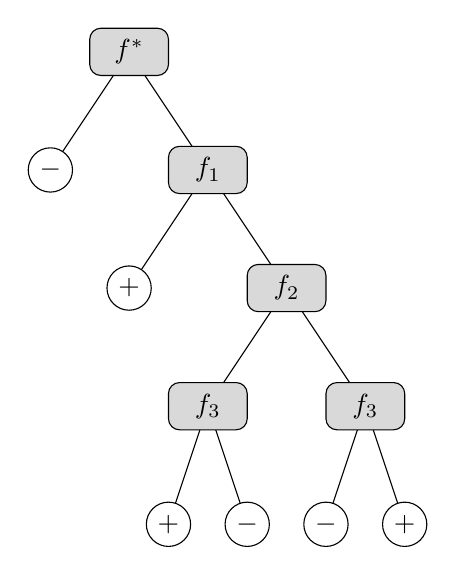
\begin{tikzpicture}[scale=1]
\draw (0,0.5)--(1,2)--(2,0.5)--(1,-1) (2,0.5)--(3,-1)--(4,-2.5)--(4.5,-4) (1.5,-4)--(2,-2.5)--(2.5,-4) (2,-2.5)--(3,-1) (3.5,-4)--(4,-2.5);
\draw[rounded corners,fill=gray!30!white] (0.5,1.7) rectangle (1.5,2.3) {};
\draw[rounded corners,fill=gray!30!white] (1.5,0.2) rectangle (2.5,0.8) {};
\draw[rounded corners,fill=gray!30!white] (2.5,-1.3) rectangle (3.5,-0.7) {};
\draw[rounded corners,fill=gray!30!white] (1.5,-2.8) rectangle (2.5,-2.2) {};
\draw[rounded corners,fill=gray!30!white] (3.5,-2.8) rectangle (4.5,-2.2) {};
\draw[fill=white] (0,0.5) circle (8pt) (1,-1) circle (8pt) (1.5,-4) circle (8pt) (2.5,-4) circle (8pt) (3.5,-4) circle (8pt) (4.5,-4) circle (8pt);
\node at (1,2) {$f^*$};
\node at (2,0.5) {$f_1$};
\node at (0,0.5) {$-$};
\node at (1,-1) {$+$};
\node at (3,-1) {$f_2$};
\node at (2,-2.5) {$f_3$};
\node at (4,-2.5) {$f_3$};
\node at (1.5,-4) {$+$};
\node at (2.5,-4) {$-$};
\node at (3.5,-4) {$-$};
\node at (4.5,-4) {$+$};
\end{tikzpicture}
\end{minipage}
\caption{} %\label{fig:example}
\end{figure}


\begin{lemma}\label{lem:umss}
The features in $\{f_1,\ldots,f_k\}$ form the only minimal support set in $S=\{f_1,\ldots,f_k,f^*\}$ for $E_k$.
\end{lemma}

\begin{proof}
First we show that $\{f_1,\ldots,f_k\}$ is a support set: let $e^-\in E^-_k$ and $e^+\in E^+_k$, by construction there is one feature $f\in \{f_1,\ldots,f_k\}$ where $f(e^+)\neq f(e^-)$. 
Now it is time to show that, for any $i\in [k]$, the set $S_i=\{f_1,\ldots,\overline{f_i},\ldots,f_k,f^*\}=S\setminus \{f_i\}$ is not a support set for $E_k$. 
For $i\in [k-2]$, let $e^-_i$ and $e^+_i$ be the negative and the positive examples such that $f(e^-_i)=f(e^+_i)=1$ if $k$ is odd ($=0$ if $k$ is even) for every $f\in S_i$: 
$e^-_i$ and $e^+_i$ can not be distinguished by a feature in $S_i$ and so $S_i$ is not a support set (note there is one such pair $exam(E_k)$). 
For $i\in \{k-1,k\}$, let $e^-_i$ and $e^+_i$ be the negative and the positive examples in $D_k$ such that $f(e^-_i)=f(e^+_i)$ for every $f\in S_i$: $e^-_i$ and $e^+_i$ can not be distinguished by a feature in $S_i$ and so $S_i$ is not a support set (note there are two of such pairs in $exam(E_k)$).
\end{proof}

\begin{lemma}\label{lem:omss}
A reduced DT $T$ with features in $\{f_1,\ldots,f_k\}$ is a DT for $E_k$ if and only if $T$ is a complete DT of height $k+1$. In particular such DT has $2^{k+2}-1$ nodes ($2^{k+1}-1$ of those are inner nodes).
\end{lemma}

\begin{proof}
In this proof we assume that a leaf is either positive or negative depending on the parity of the number of right arcs present in the unique path from the root to that leaf. We start with the forward direction: let $T$ be a reduced DT that is not a complete DT of height $k+1$. Let $P$ a path of $T$ from the root to a leaf $\ell$ of length at most $k$: at most $k-1$ features appear in $P$ and so there exists a feature $f_i\in \{f_1,\ldots,f_k\}$ that does not appear in $P$. Since $S_i$ is not a support set for $E$, there exit a negative example $e^-$ and a positive example $e^+$ that can not be distinguished by $S_i$, this means that $\{e^-,e^+\}\subseteq E_T(\ell)$ and so $T$ is not a DT for $E_k$. 

In order to prove the backward direction, we assume that $T$ is a reduced and complete DT of height $k+1$ with features in $\{f_1,\ldots,f_k\}$. Let $P$ be a path of $T$ from the root to a leaf $\ell$ of length $k+1$. Since $T$ is reduced, every feature of $\{f_1,\ldots,f_k\}$ appears exactly once in $P$. Since $\{f_1,\ldots,f_k\}$ is a support set, there is only one example $e_\ell$ that ends $\ell$, that is $e_\ell\in E_T(\ell)$. From this proof, it follows that every reduced DT $T$ with features in $\{f_1,\ldots,f_k\}$ for $E_k$ has $2^{k+2}-1$ nodes ($2^{k+1}-1$ of those are inner nodes).
\end{proof}

Let $\sigma$ be any bijection of the set $[k-2]$ and $\tau$ be any of the two bijections of the set $\{k-1,k\}$ and (arbitrarily) define $\sigma(k-1)=\tau(k-1)$. Let us describe a DT $T_{\sigma,\tau}$ as follows. The root of $r$ has feature $f^*$. The left child of $r$ is a negative leaf and the right child $v_1$ has feature $f_{\sigma(1)}$. For every $i\in [k-2]$, the left child of $v_i$ is a positive leaf and the right child $v_{i+1}$ has feature $f_{\sigma(i+1)}$. Finally $v_k$ and $v'_k$ are respectively the left and right child of $v_{k-1}$, both having feature $f_{\tau(k)}$. The children of $v_k$ and $v'_k$ are leaves that are either positive or negative depending on the parity of the number of right arcs present in the unique path from the root to that leaf.
In particular note that $T_{\sigma,\tau}$ has $2k+5$ nodes ($k+2$ of those are inner nodes).

\begin{lemma}\label{lem:emss}
A DT $T'$ is a DT for $E_k$ of minimum size among those with features in $\{f_1,\ldots,f_k,f^*\}$ if and only if $T'=T_{\sigma,\tau}$, for some permutation $\sigma$ and $\tau$.
\end{lemma}

\begin{proof}
We start by doing the forward direction: TO DO

\smallskip
In order to prove the backward direction, we assume that $T'=T_{\sigma,\tau}$, for some permutation $\sigma$ and $\tau$. By construction, $r$ and its feature $f^*$ send every negative example to its left child $c_\ell$, which is a negative leaf, except for the two negative examples in $D_k$, that is, if $\{e_1^-,e_2^-\}=E^-_k\cap D_k$ then $E_{T'}(c_\ell)=E^-_k\setminus \{e_1^-,e_2^-\}$ and $E_{T'}(v_1)=E^+_k\cup \{e_1^-,e_2^-\}$.

Let $e$ be an example in $D_k$; by construction, for every $i\in [k-2]$ if $e\in  E_{T'}(v_i)$ then $e\in E_{T'}(v_{i+1})$ and by induction we obtain that $e\in E_{T'}(v_{k-1})$. Let $e$ be an example in $\overline{D_k}$ and $j\in [k-2]$ be the minimum integer such that $f_{\sigma(j)}(e)=0$. This means that $e\not\in E_{T'}(v_{j+1})$ and $e$ is classified by the left child of the node $v_j$. We have just proved that $D_k=E_{T'}(v_{k-1})$ and that $T'$ classifies $\overline{D_k}$. Now it is straightforward to show that $T'_{v_{k-1}}$ classifies $D_k$.

Finally we have to show that $T'=T_{\sigma,\tau}$ has minimum size. Let $T''$ be a reduced DT for $E_k$ with features in $\{f_1,\ldots,f_k,f^*\}$. If $T''$ does not have a node with feature $f^*$, then by Lemma~\ref{lem:omss} $|T''|>|T_{\sigma,\tau}|$. Let $v^*$ be a node in $T''$ with feature $f^*$. Since the set of features of a DT for $E_k$ has to be a support set, thanks to Lemma~\ref{lem:umss} we can assume that $feat(T'')=\{f_1,\ldots,f_k,f^*\}$. Let $j$ be the minimum level in which there is a node with feature in $\{f_{k-1},f_k\}$. First, let us assume $v^*$ is the root of $T''$. If $j\geq k-1$, then it is easy to see that $T''=T_{\sigma,\tau}$ for some bijections $\sigma$ and $\tau$ and so $|T''|=|T_{\sigma,\tau}|$. If $j\in \{2,\ldots,k-2\}$ TO CONTINUE




\end{proof}





\subsection{For Height}

For every natural number $k\geq 1$, we can define a CI $E_k$ as follows. Let $E_k$ be the CI with exactly $2^k$ examples $\{e_1,\ldots,e_{2^k}\}$ on $k$ binary features $\{f_1,\ldots,f_k\}$: there is exactly one example for every of the $2^k$ feature assignments.
An example $e\in exam(E_k)$ is a positive example if $|\{f\in feat(E_k)~|~f(e)=1\}|$ is even and negative otherwise.

Let {\sc in} be a subset of examples in $exam(E_k)$ that can be classified by a DT $T_\text{{\sc in}}$ of height $log(k)$ and denote by {\sc out} all the remaining examples, that is {\sc out}$=exam(E_k)\setminus$ {\sc in}. Now we are ready to define a new feature $f'$ follows:$f'(e)=0$ if $e\in$~{\sc in} and $f'(e)=1$ otherwise. We also introduce another new feature $f''$ as follows: $f''(e)=0$ if either $e\in$~{\sc in} or $e$ is a negative example and $f''(e)=1$ otherwise.

\begin{lemma}\label{lem:humss}
The features in $\{f_1,\ldots,f_k\}$ form the only minimal support set in $S=\{f_1,\ldots,f_k,f',f''\}$ for $E_k$.
\end{lemma}

\begin{proof}
By Lemma~\ref{lem:umss}, the set $\{f_1,\ldots,f_k\}$ is a support set.
Now it is time to show that, for any $i\in [k]$, the set $S_i=\{f_1,\ldots,\overline{f_i},\ldots,f_k,f',f''\}=S\setminus \{f_i\}$ is not a support set for $E_k$. 


%For $i\in [k-2]$, let $e^-_i$ and $e^+_i$ be the negative and the positive examples such that $f(e^-_i)=f(e^+_i)=1$ if $k$ is odd ($=0$ if $k$ is even) for every $f\in S_i$: $e^-_i$ and $e^+_i$ can not be distinguished by a feature in $S_i$ and so $S_i$ is not a support set (note there is one such pair $exam(E_k)$). 
%For $i\in \{k-1,k\}$, let $e^-_i$ and $e^+_i$ be the negative and the positive examples in $D_k$ such that $f(e^-_i)=f(e^+_i)$ for every $f\in S_i$: $e^-_i$ and $e^+_i$ can not be distinguished by a feature in $S_i$ and so $S_i$ is not a support set (note there are two of such pairs in $exam(E_k)$).
\end{proof}





\begin{figure}[h]
\small
\begin{minipage}{0.33\linewidth}
\centering
\begin{tabular}{ccc|c|c|cc}
$f_1$ & $f_2$ & $f_3$ & $f'$ & $f''$ &\\
\hline
$0$ & $0$ & $0$ & $0$ & $0$ & $+$ \\
$0$ & $0$ & $1$ & $0$ & $0$ & $-$ & {\sc in}\\
$1$ & $0$ & $0$ & $0$ & $0$ & $-$ \\
\hline
$0$ & $1$ & $0$ & $1$ & $0$ & $-$ \\
$0$ & $1$ & $1$ & $1$ & $1$ & $+$ \\
$1$ & $0$ & $1$ & $1$ & $1$ & $+$ & {\sc out}\\
$1$ & $1$ & $0$ & $1$ & $1$ & $+$ \\
$1$ & $1$ & $1$ & $1$ & $0$ & $-$
\end{tabular}
\end{minipage}%
\begin{minipage}{0.7\linewidth}
\centering
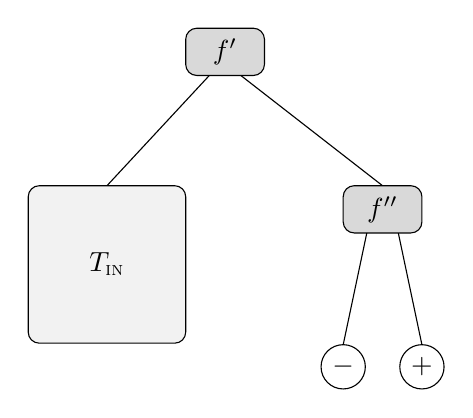
\begin{tikzpicture}[scale=1]
\draw (0.2,1.7)--(2,0.3) (-0.2,1.7)--(-1.5,0.3) (1.8,-0.3)--(1.5,-1.72) (2.2,-0.3)--(2.5,-1.72);
\draw[rounded corners,fill=gray!30!white] (-0.5,1.7) rectangle (0.5,2.3) {};
\draw[rounded corners,fill=gray!30!white] (1.5,-0.3) rectangle (2.5,0.3) {};
\draw[rounded corners,fill=gray!10!white] (-2.5,-1.7) rectangle (-0.5,0.3) {};
\draw (1.5,-2) circle (8pt);
\draw (2.5,-2) circle (8pt);
\node at (0,2) {$f'$};
\node at (2,0) {$f''$};
\node at (-1.5,-0.7) {$T_\text{{\sc in}}$};
\node at (1.5,-2) {$-$};
\node at (2.5,-2) {$+$};
\end{tikzpicture}
\end{minipage}
\caption{} %\label{fig:example}
\end{figure}








\bibliography{literature}
\end{document}